\chapter{Implementation}

The goal of POOP-SNOOP is to provide an interface that motivates non-scientist citizens to solve puzzles to further the knowledge base created by the Biology Department at Cal Poly, their work gathering and pyroprinting E. coli, and analyzing that information with various tools including CPLOP. 

From the beginning, the goal was to introduce exaggerated juiciness into a citizen science game. The core mechanic of POOP-SNOOP is simple and there is plenty of room for modification many possible directions. A web browser based game was chosen to maximize possible participation; the prototypes are both created using vectorized graphics with help from a basic tweening library. 

The most popular citizen science projects are hosted on Zooniverse \cite{borne2011zooniverse}, who indicate that over one million participants have helped solve science with their website although Zooniverse is a collection of dozens of games from a variety of research projects and designers \cite{borne2011zooniverse}. On the other hand, Fold-it requires an installation and claims 57,000 have participated \cite{cooper2010challenge}.

\section{Mechanics} 

The puzzle itself is very reminiscent of the spreadsheet biologists originally manipulated to visually identified strains.

\subsection{Modified self-similarity matrix}

The original spreadsheet consisted of E. coli isolates organized into a self-similarity matrix of isolates in each row and column. The intersection between a row and a column compared the two isolates; a self-similarity matrix to compares a dataset to itself. To identify strains within a dataset, both the 16S-23S region and the 23S-5S regions of each pyroprint. In the standard self-similarity matrix, there are two comparisons between each different member of the dataset. Each E. coli isolate must be compared on both the 16S-23S region and the 23S-5S region to be considered in the same strain, therefore by modifying the self-similarity matrix to account for these two different comparisons the modified self-similarity matrix satisfies our requirement.

Every E. coli isolate in our dataset is compared to each other dataset twice--one comparison between the 23S-5S region and one comparison between the 16S-23S region. E. coli isolates are compared to themselves once, but must be in the same strain as themselves by identity. 

The self-similarity matrix must maintain the same order and length in both dimensions. An E. coli isolate is always compared to itself along the diagonal.

The comparison between two regions of DNA in an isolate is represented by a value between 0 and 1. The threshold for strain similarity is a comparison value of 0.95 or greater, and a strain can only consist of E. coli isolates that each compare about the strain similarity threshold on both regions of compared DNA. See section \ref{strain-identification} for more detail.

\subsection{Identifying strains}

Originally, identifying strains was the process of manually swapping two columns then carefully swapping the corresponding two rows to maintain the self-similarity matrix. Strains emerge when perfectly square clusters of DNA comparisons align along the diagonal. Metaphorically this indicates that each isolate in the indicated rows (the columns are the same isolates) could be in a strain together.

The goal of POOP-SNOOP is to encourage players to try different organizations of the puzzle to find the best possible strain. The possible solution set size is n-squared, which could be easily traversed algorithmically. This game is completely unnecessary, but an example of a potential scientific discovery puzzle game.

\section{POOP-SNOOP}

\begin{table}
\begin{center}

\begin{tabular}{|>{\centering}p{3cm}|>{\centering}p{5cm}|>{\centering}p{5cm}|}
\hline 
Category&  Juicy&  Juiceless
\tabularnewline
\hline 

Puzzle initialization&  Puzzle descends into place&  No animation
\tabularnewline
\hline 

Mousedown row/column&  Bouncing animation, simulated depth&  Black outline
\tabularnewline
\hline 

Mouseover row/column&  Indicator animation pointing in direction of travel&  Black indicator
\tabularnewline
\hline 

Dragging row/column&  Other rows slide into new position&  No animation
\tabularnewline
\hline 

Mouseup row/column&  Animation highlighting scored cluster, background effects&  No animation
\tabularnewline
\hline 

Tutorial text&  Slides and fades, fonts, positioning&  No animation
\tabularnewline
\hline

Tutorial slides& Various animations per slide&  No animation
\tabularnewline
\hline

\end{tabular}

\caption[``Juicy" elements of POOP-SNOOP prototypes]{Summary of differences between ``juicy" and ``juiceless" POOP-SNOOP puzzle and tutorial.}
\label{table:juice}
\end{center}
\end{table}

The essential mechanic of POOP-SNOOP is essentially reordering objects in a single dimensional list while observing their relationship with its local cluster. This data is easily represented as a spreadsheet-like grid such that players can associate with the datastructure.

Unlike many games including Fold-it \cite{cooper2010challenge} or Juicy Breakout \cite{juiceitorloseit}, there isn't a specific physical metaphor for a real object that POOP-SNOOP is emulating. A spreadsheet can be thought of as a grid, or a matrix, but other than in computer applications people do not often deal with these structures. Still, in order to make this game enticing, design hints needed to be incorporated.

\subsection{The Grid}

\begin{figure}
\begin{center}
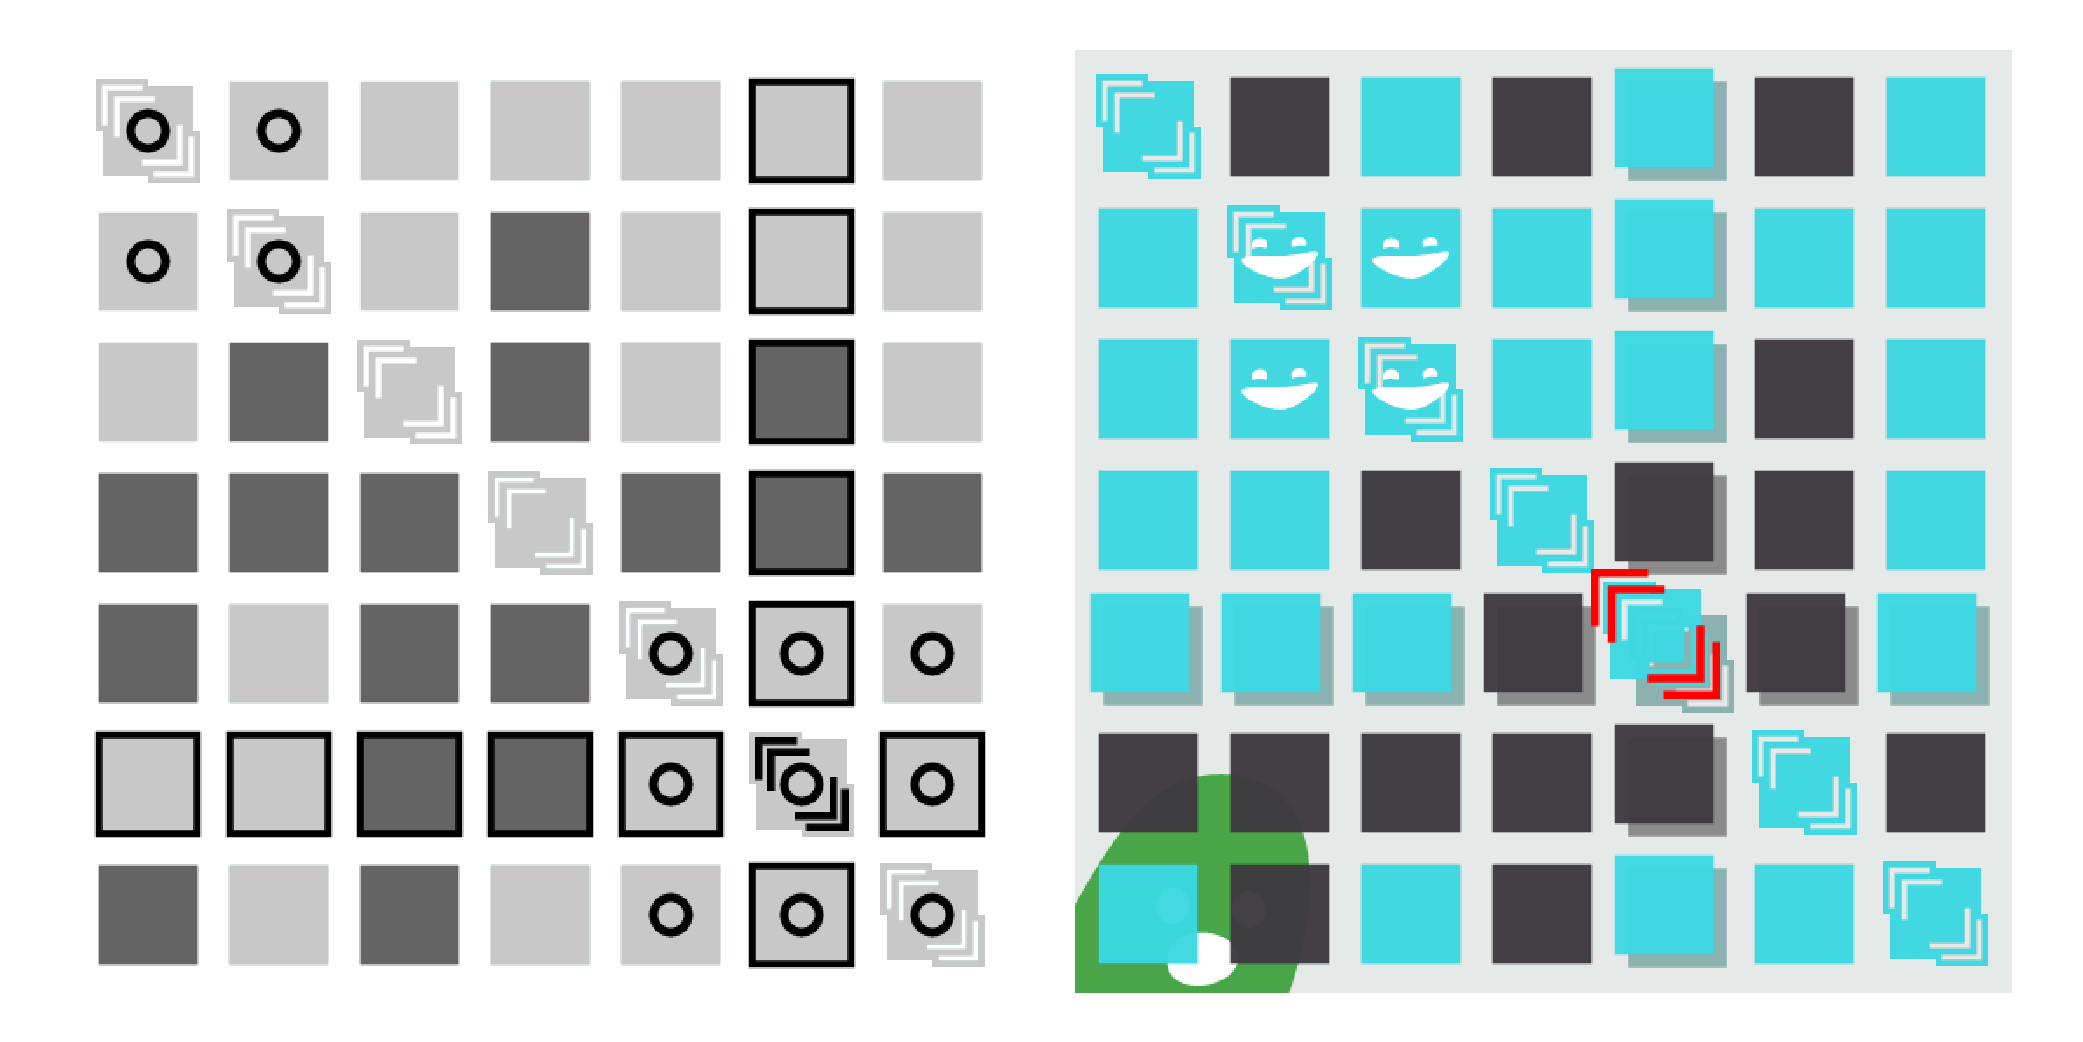
\includegraphics[width=150mm]{images/grid.pdf}
\caption[Differences between game layout in each prototype]{The left image is the ``juiceless" prototype. Circles indicate the current solution, black outline indicate the selected row/column pair. On the right is the ``juicy" prototype with the selected row/column pair.}
\label{fig:grid}
\end{center}
\end{figure}

Spreadsheets remind players of work and many people associate games in a completely different category than work. To incorporate the grid structure of spreadsheets without the work, the design followed a clean grid structure. Elements in the grid are the same size to represent that they are essentially representations of the same objects in our puzzle. The simulated space of POOP-SNOOP should imply a table or flat plain surface which doesn't interfere with the puzzle. In figure \ref{fig:grid}, each comparison between isolates is represented by a block--light gray is matching, dark gray is not matching.

Though it was originally a bit sarcastic, Petri Puhro \cite{juiceitorloseit} suggested personality by adding faces and adjusting their eyes to elicit emotional response. In figure \ref{fig:grid}, comparisons in the ``juicy" prototype contributing to the solution are given a smiling face. The faces of the boxes are visible when they are part of a larger cluster. The intent is that the player would be encouraged to put as many ``happy" blocks together to find the largest solution. In the non-juicy version, dark circles indicated cells that were part of a solution.

\subsection{Interaction}

Players need to reorganize the grid easily and play with its orientation. The most fundamental metaphor for this in computer applications is clicking and dragging. If a computer user were to click an icon from the desktop and drag it, they could change its position. Unfortunately, the relationships in the grid require that the entire row and column move with it. Without explicitly connecting them in some way, the intent is that players would be able to observe the results of their action as part of the real-time feedback loop and learn the mechanic this way. As players click and drag, the grid reorganizes around them to immediately reflect the implications of their decision.

\begin{figure}
\begin{center}
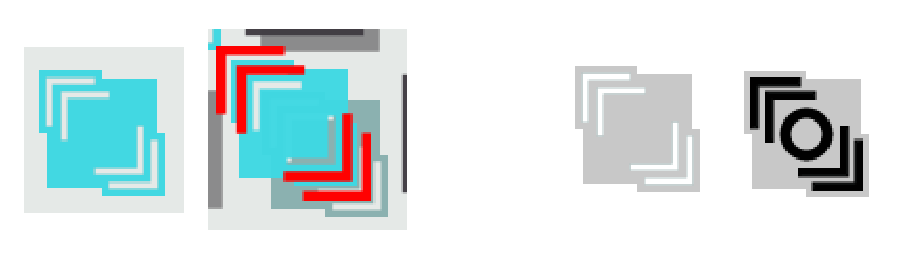
\includegraphics[width=100mm]{images/chevron.pdf}
\caption[Differences between chevrons in each prototype]{On the left, ``juicy" chevrons when unselected and selected. On the right, ``juiceless" chevrons when unselected and selected.}
\label{fig:chevrons}
\end{center}
\end{figure}

The ability to drag squares should be made obvious to players. The pieces of the grid are all important to the current and possible solutions, but only the pieces along the diagonal are interactive. To exhibit this characateristic, chevrons pointing in their potential range of travel were added. The chevrons intended to manipulate a physically rough surface or small bumps and the arrows indicated movement. In figure \ref{fig:chevrons}, the differences between the ``juicy" chevron and ``juiceless" chevron are demonstrated; the juicy chevron is animated.

In ``juicy" POOP-SNOOP, each box has a shadow and pops up off the plane of the rest of the grid when moused over. A simple opacity and shadow gives the pieces of the puzzle depth when rows intersect slightly as players rearrange the puzzle. While moving the puzzle, players can see other pieces through theirs, adding to the illusion of depth. Overall, it resemebles the metaphore for small, translucent pieces of paper. The rows and cells of the grid bounce up into a hover state as they become activated which is playful, but subtle enough to not be overwhelming. As the player actively rearranges the puzzle, they are given visual hints about their actions because the rows slide gently into their new place, rather than simply appearing in their new position. Because the movement of the rows and columns is unnatural, this behavior intends to reinforce the mechanic for new players. The objects in POOP-SNOOP do not interact with eachother, but slide past one another.

As the boxes of the grid move, their motion is subtley enhanced by stretching and squeezing the direction of their movement. It is especially difficult to see how the puzzle changes when a column and row change orientation.

\subsection{Scoring}

Scientific discovery games exist because researchers do not know the solution to the given puzzle. Players would not normally know the solution of a POOP-SNOOP puzzle, but a message that alerted users when they solved the introductory level. In the nature of ``juicy" design, the intent was that players would be given clues other than a number to indicate their score. The size of the score itself is a very visual representation of score.

Rearranging the puzzle consisted of a mousedown action to enable dragging, dragging the mouse to move the row-column pair, then releasing the mouse to return the grid to a resting state. As the player released their currently selected row, the intention of the game was to respond to that change and convey the current score to the player. Cluster highlighting happened simultaneously with background effects.

Background effects are designed reward positive player behavior with exciting explosions, colors, and motion. The goal of the effects is to encourage players to keep trying new combinations and working towards the best possible solution. The effects were designed to give more feedback for larger, better solutions and less feedback for smaller solutions. Five separated effects consisting of geometric shapes and patterns animated and exploded when dragging was complete and the score was totalled; an example of these effects can be seen in figure \ref{fig:background}. The background effects lasted about two seconds and interrupted gameplay because the puzzle was hdiden. Players were able to click and end the animation early, but it was not made obvious.

\begin{figure}
\begin{center}
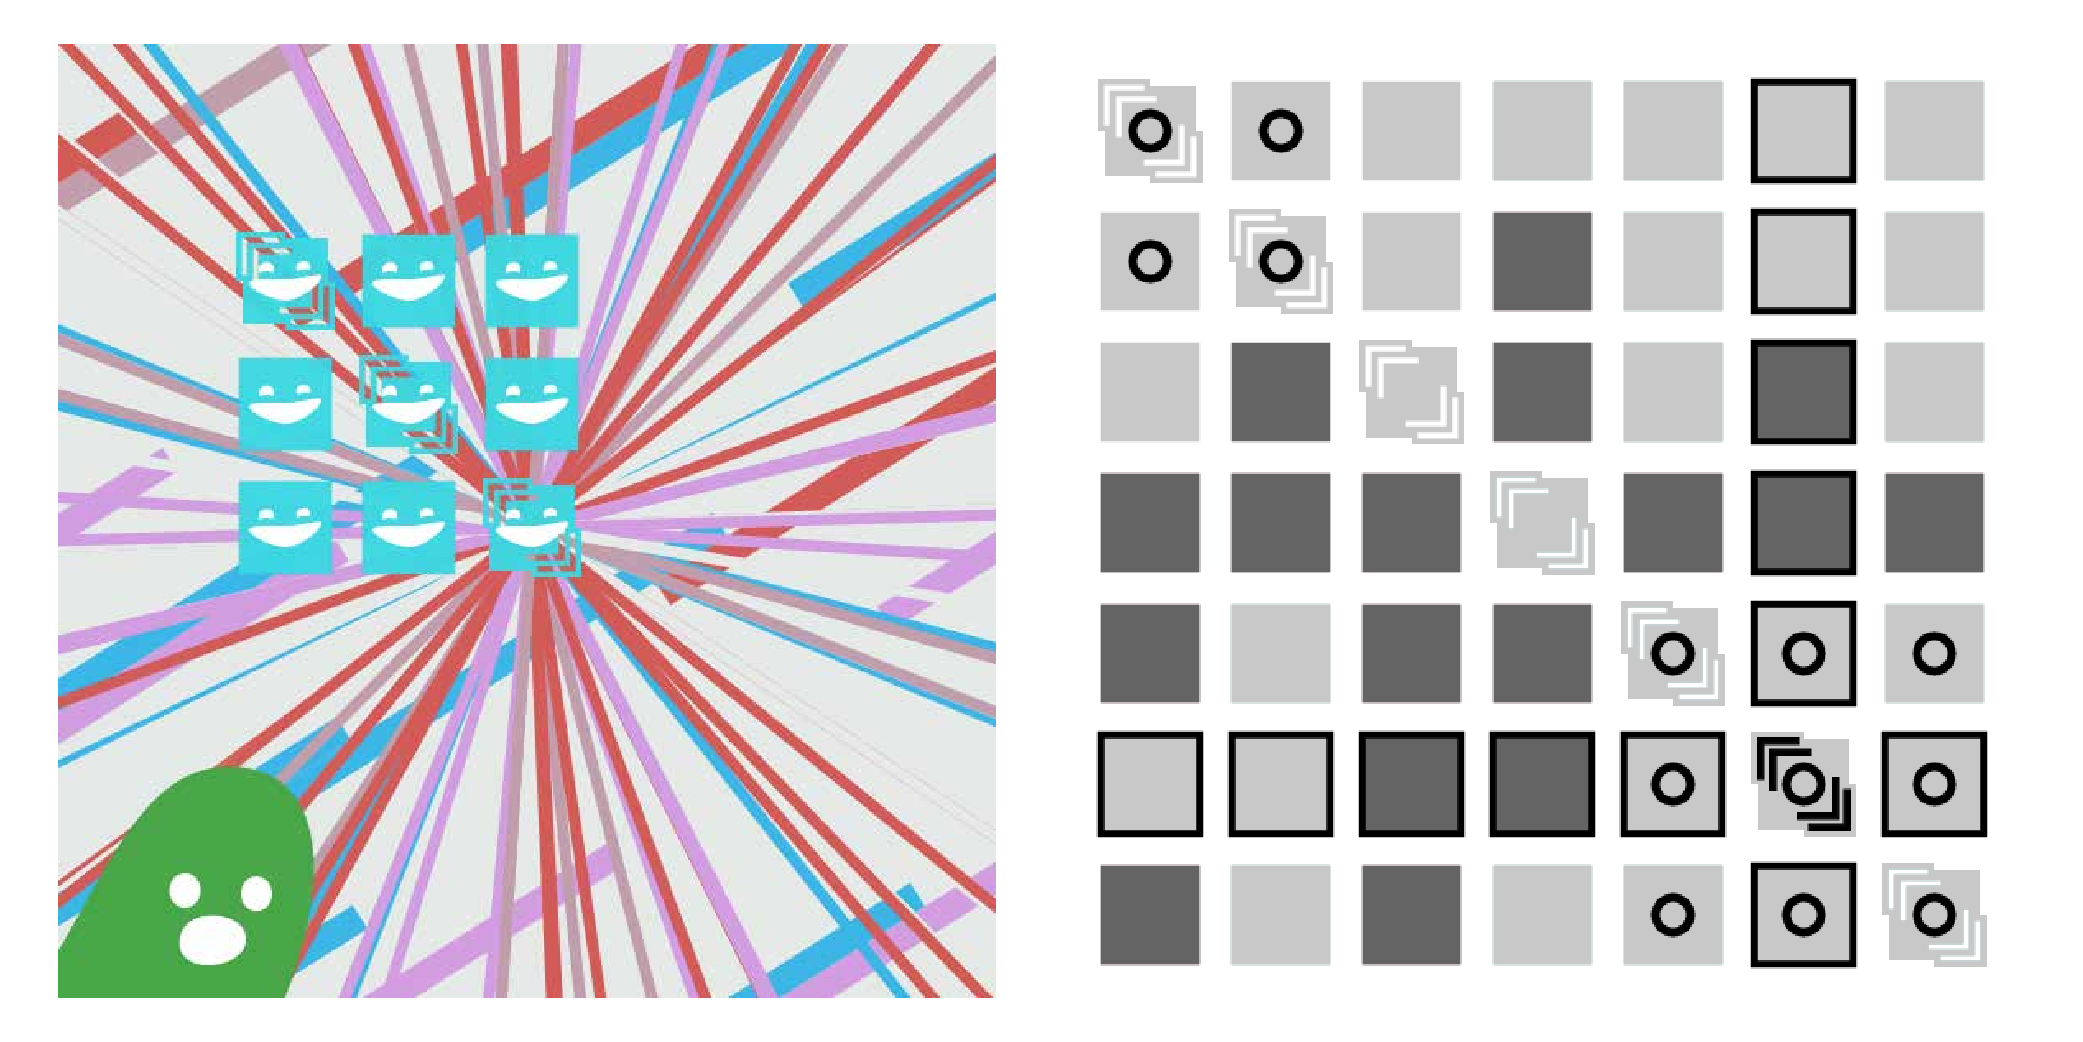
\includegraphics[width=150mm]{images/background.pdf}
\caption[Differences between animations in each prototype]{On the left, the animation when completing a drag in the ``juicy" prototype. On the right, the same event in the ``juiceless" prototype.}
\label{fig:background}
\end{center}
\end{figure}

\section{Tutorial}

POOP-SNOOP requires a tutorial. Feedback during the design phase indicated that the scientific knowledge helped players understand why they were essentially reorganizing a grid. The mechanics themselves were confusing and unintuitive to new players. Like other scientific discovery games, the tutorial is the first section of the game that people interact with, but does ``juicy" design have implications here? Each version of POOP-SNOOP was tested with a prototypical tutorial.

The content of the tutorials was designed to be identical; each tutorial had the same illustrations, same text, and the same order. Within the tutorial, players interacted with a small version of POOP-SNOOP. The ``juicy" version of the tutorial also contained the ``juicy" version of POOP-SNOOP and vice versa. The ``juicy" version was given some design thought. The placement of text, color, and overall feel was augmented to measure its effect on learning. One slide from both versions of the tutorial are shown in figure \ref{fig:tutorial}.

\begin{figure}
\begin{center}
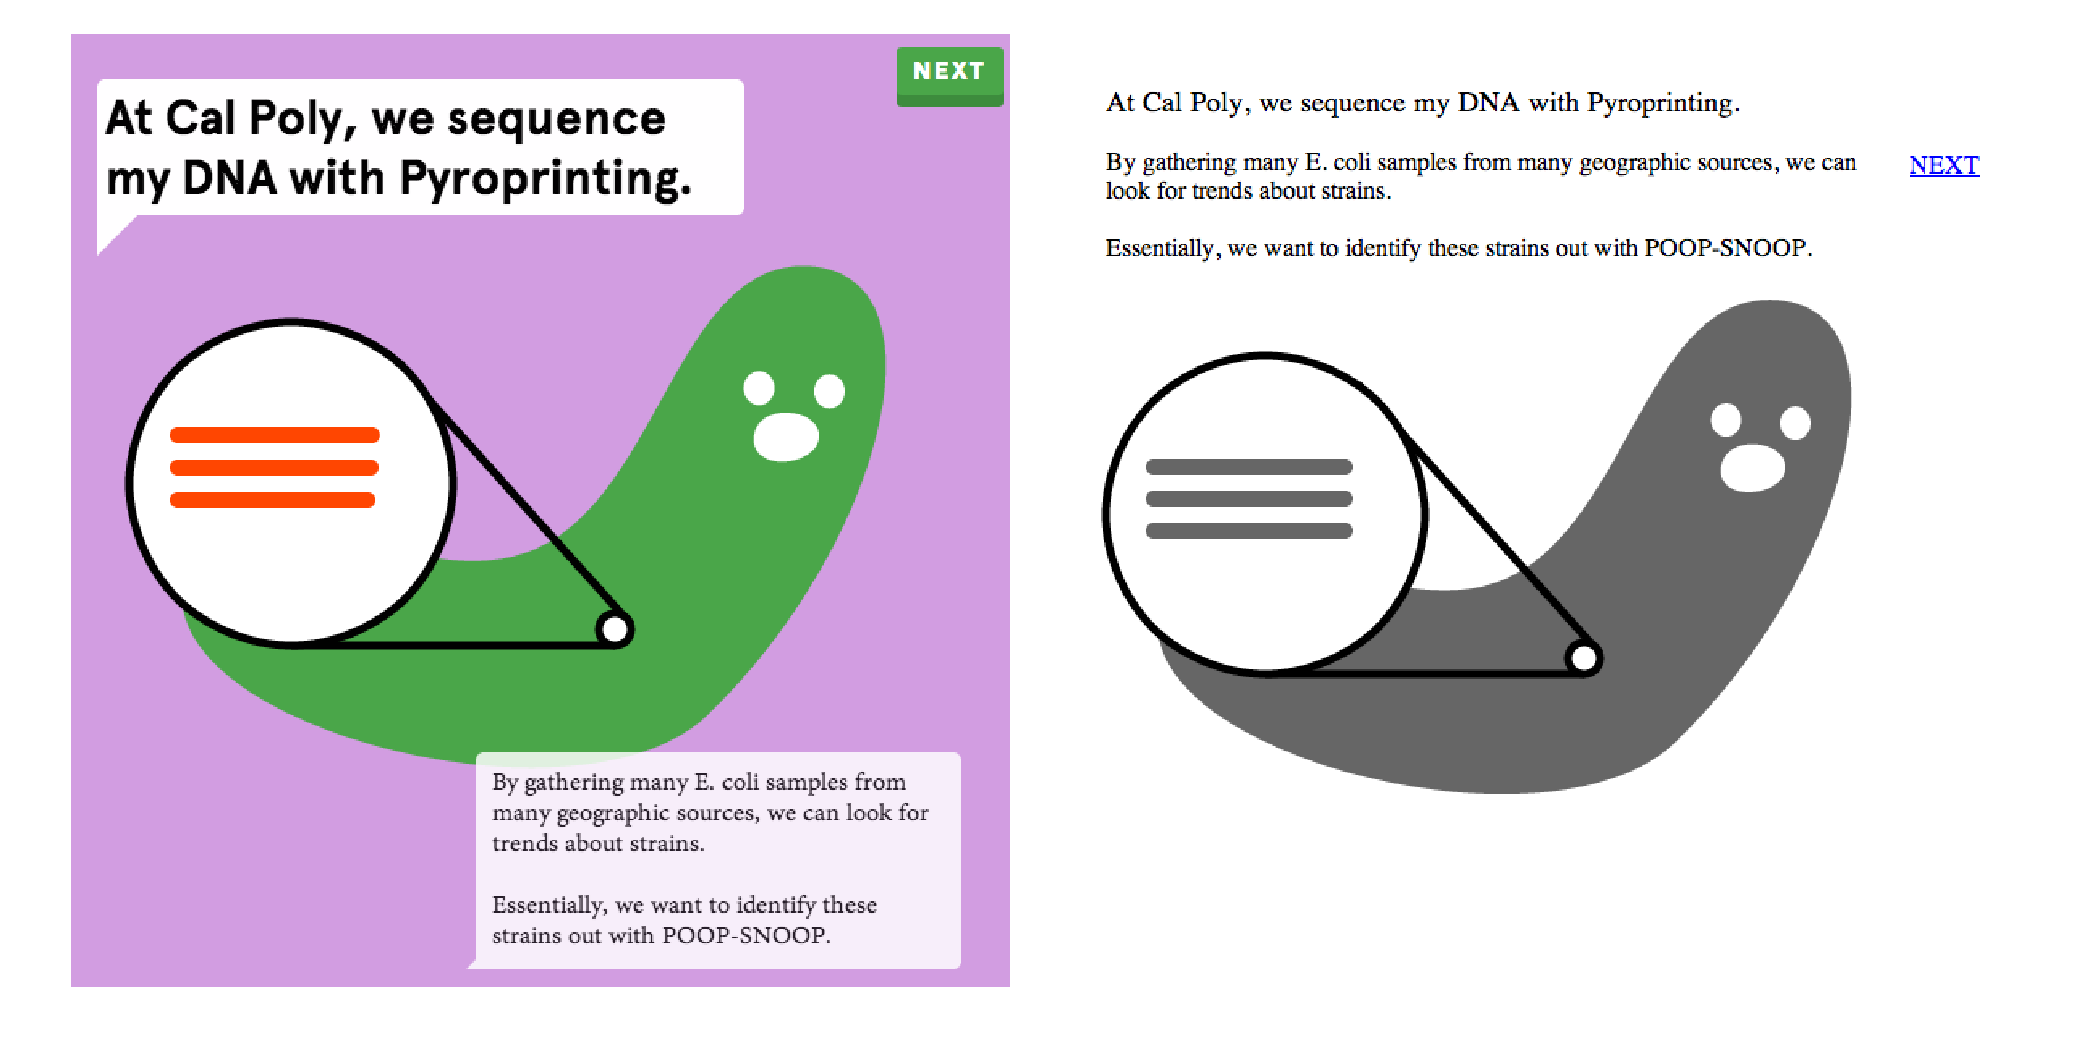
\includegraphics[width=150mm]{images/tutorial.pdf}
\caption[Differences between tutorials in each prototype]{On the left and right, an example of the ``juicy" tutorial and ``juiceless" tutorial, respectively.}
\label{fig:tutorial}
\end{center}
\end{figure}

\subsection{Text}

In order to entice players to read the text and digest the scientific concepts, text in the ``juicy" tutorial assumed the metaphor of speech bubbles being recited by an E. coli character. The intent of this design was that players would associate the character as guiding them in the tutorial. Special text effects should encourage player engagement. 

\subsection{Animations}

Both versions of the tutorial had the same content, but the ``juicy" version of the puzzle would often introduce content in a more appealing way. The DNA slide ``spun" into view and the lines indicating a ``match" were animated and bouncing. As POOP-SNOOP was introduced it gently slid down into the player's space, whereas the puzzle simply appeared in the ``juiceless" version.
